\section{Background} 

\subsection{Approximate Computing}
Approximate computing is known under many names including transprecision computing, mixed-precision computing, reduced precision computing, ...
All these concepts unite under the goal of trying to gain better resource usage or computation speed from reducing the precision of calculations in the program. 

Approximate computing does not require any special tooling to implement. Some tricks, such as memoization (caching results of expensive computations) or loop perforation, or just using types with less bits (float instead of double, i32 instead of i64 etc.) can be performed by the programmer directly in code. Doing all this manually however requires the program composer to instrument the program to verify that the output is within the required bounds of precision, and whether any of the steps taken makes the program behave in an unexpected fashion. For this reason there have been created several tools aimed at research on the utility of approximate computing that encompasses both the execution of the code and verification of the results. 

%figures of approximate computing techniques?
\subsubsection{Approximate computing through reducing amount of bits}

This thesis focuses on mainly two tools: floatsmith and \taffo. In the papers describing them they are capable of reducing the precision of a program written using floating point variables through the usage of c/c++ annotations (that can normally be safely ignored), and propagates changes throughout the program without having to annotate all variables in the program.

Floatsmith aims to achieve mixed precision programs that vary the size of the floating point numbers used throughout, selecting from the IEEE 754-2008 Standard for Floating-Point Arithmetic for single- (32 bit), double- (64 bit), quad- (128 bit) and half-precision (16-bit) floating point numbers. Figure~\ref{fig:float_bit_representation} shows a bit representation of a number using the same principles as the IEEE standard, but with arbitrarily selected sizes of the different sections of the bits.
\begin{figure}
    \centering
    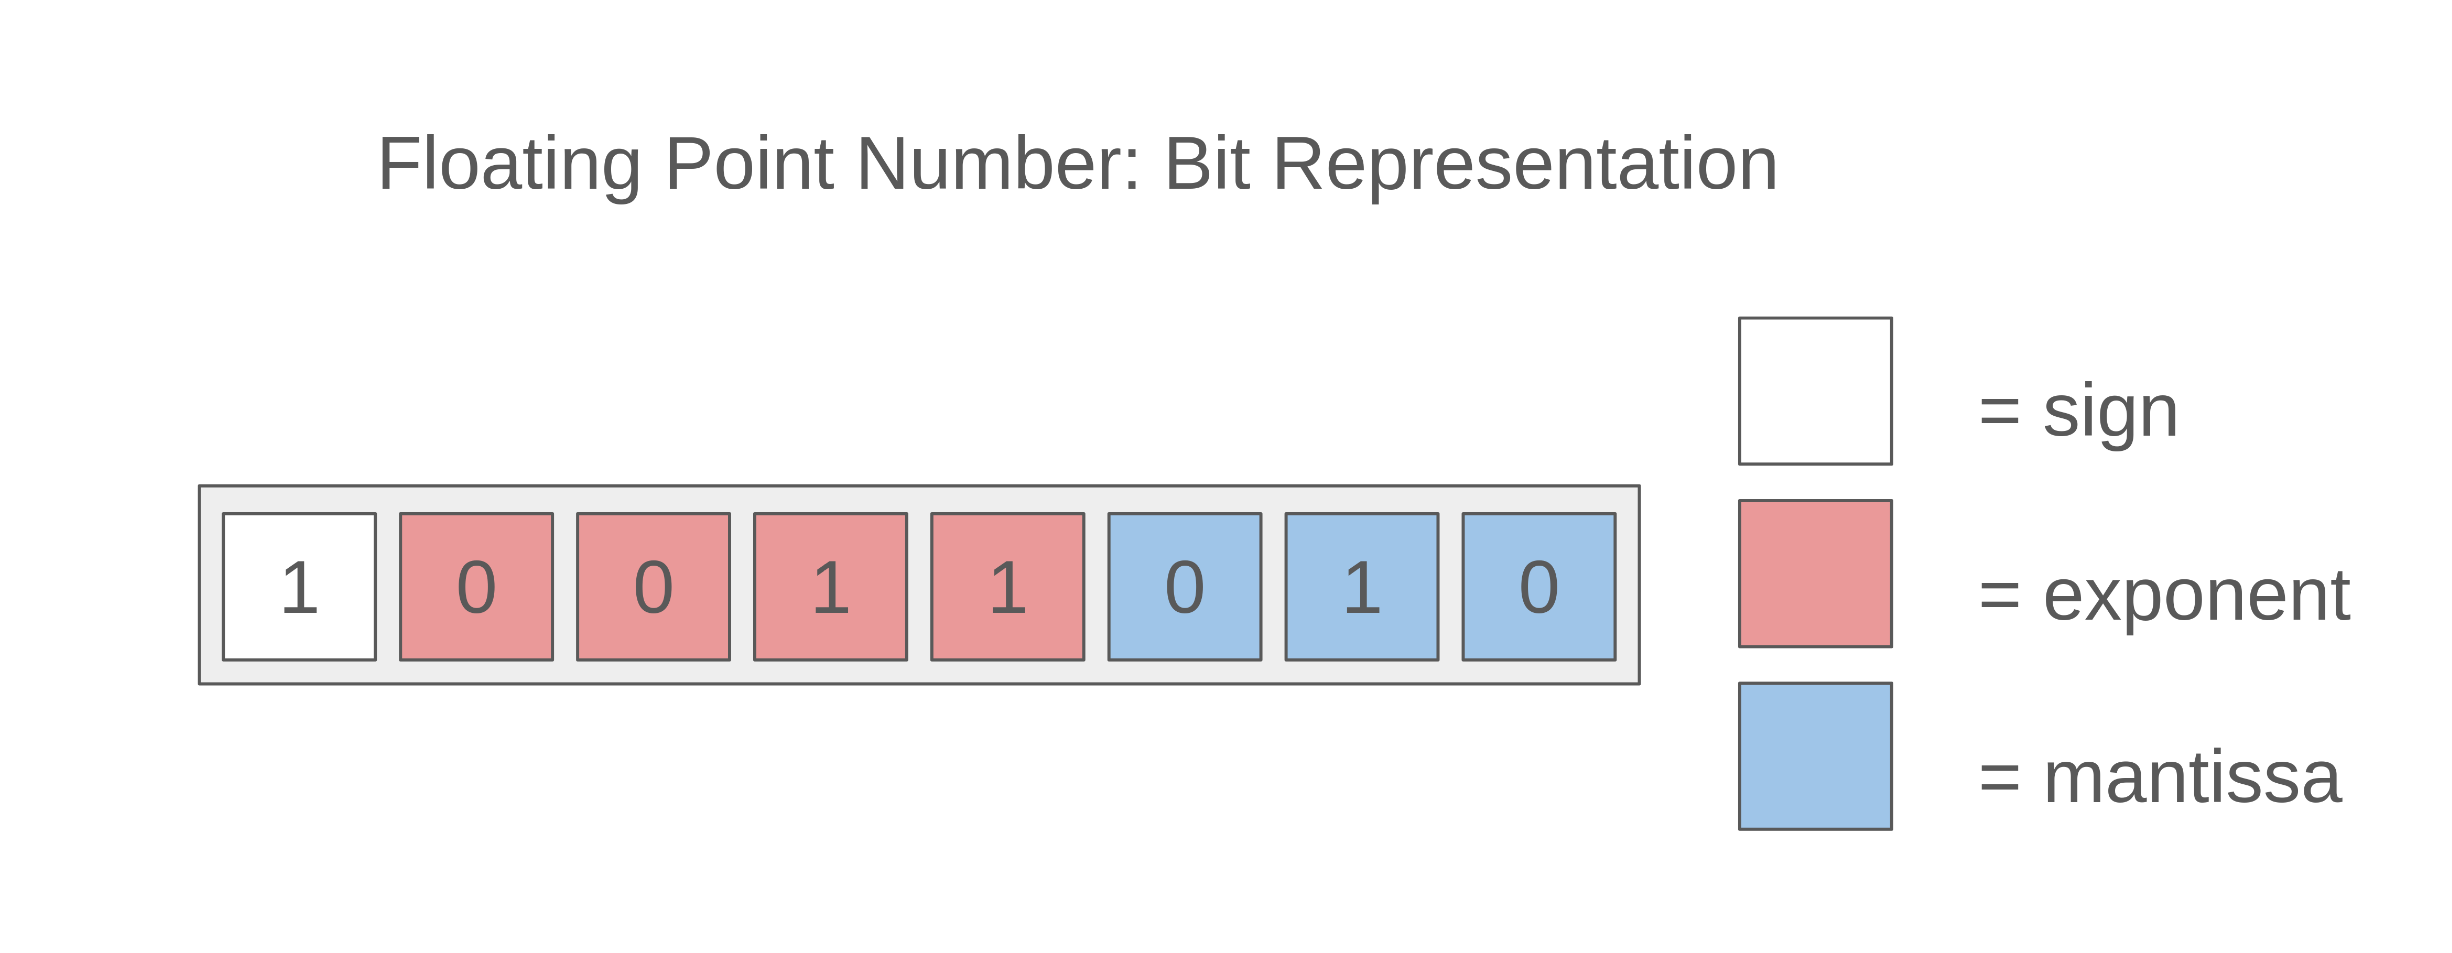
\includegraphics[width=0.5\linewidth]{Images/float_bit_representation.png}
    \caption{simplified floating point representation of a number, in this case the number 0.078125}
    \label{fig:float_bit_representation}
\end{figure}

Equation~\ref{eq:float} shows the equation that corresponds to the real value of a floating point number stored in this format.

\begin{equation}\label{eq:float}
    (-1)^{bit_7} * 2^{(exponent) - 7} * mantissa \, value
\end{equation}

The sign bit decides whether the number is positive or not. The function of the bit is shown in equation~\ref{eq:float1}.

\begin{equation} \label{eq:float1}
    (-1)^{1} = -1
\end{equation}

The exponent part of the floating point number decides the exponent part of the equation. The IEEE standard defines the exponent part of the number using an implicit negative offset, such that if all bits except the leftmost bit (bit number 6 in figure~\ref{fig:float_bit_representation}) are set to 1, the exponent is 0. For the arbitrary floating point format shown in figure~\ref{fig:float_bit_representation}, the offset becomes $2^4 - 1$, which is 7. This makes the exponent part of our arbitrary floating point number as shown in~\ref{eq:float2}.
\begin{equation} \label{eq:float2}
    2^{4-7} = 2^{-3}
\end{equation}

The final part of the floating point number, the mantissa, also known as the fraction or the significand, is usually the largest part (with respect to the amount of bits in a bitwise representation it takes up) of a floating point number, but seeing as the floating point representation in figure~\ref{fig:float_bit_representation} is entirely of my invention I don't have to conform to those norms, though I will follow the same rules for calculating the value.
The value of the number is calculated as with a bitwise represented integer, only starting at bit index 2 the bit value is $bit\,value*2^-1$, the value at bit index 1 is $bit\,value*2^-2$, and so on so forth. Additionally, an implicit value of 1 is added to the value. This makes the value represented in figure~\ref{fig:float_bit_representation} shown in~\ref{eq:float3}:

\begin{equation}\label{eq:float3}
   1 + 0*2^{-1} + 1*2^{-2} + 0*2^{-3} = 1.25
\end{equation}

Plugging in the values found above into equation~\ref{eq:float} gives us $-1 * 2^{-3} * 1.25 = 0.078125$
The IEEE definitions have additional special cases for when all bits in the exponent are either 1 or 0 to deal with special situations, but this is not important for a basic understanding of how the bit representation works.

When reducing the size of the data you are operating on, for example replacing some of the double precision floating point values to single precision floating point values, the most significant change is that you are required to fetch and store less bits from memory, alleviating the storage bottle neck in processing~\cite{floatsmith_paper}.

\taffo also performs conversions from floating point number representations, but instead of switching between different bit widths of floating point numbers, \taffo transforms numbers to fixed point representation. Figure~\ref{fig:fixed_point_representation} shows an arbitrary number, and its complement (the same number multiplied by -1) in binary.

\begin{figure}
    \centering
    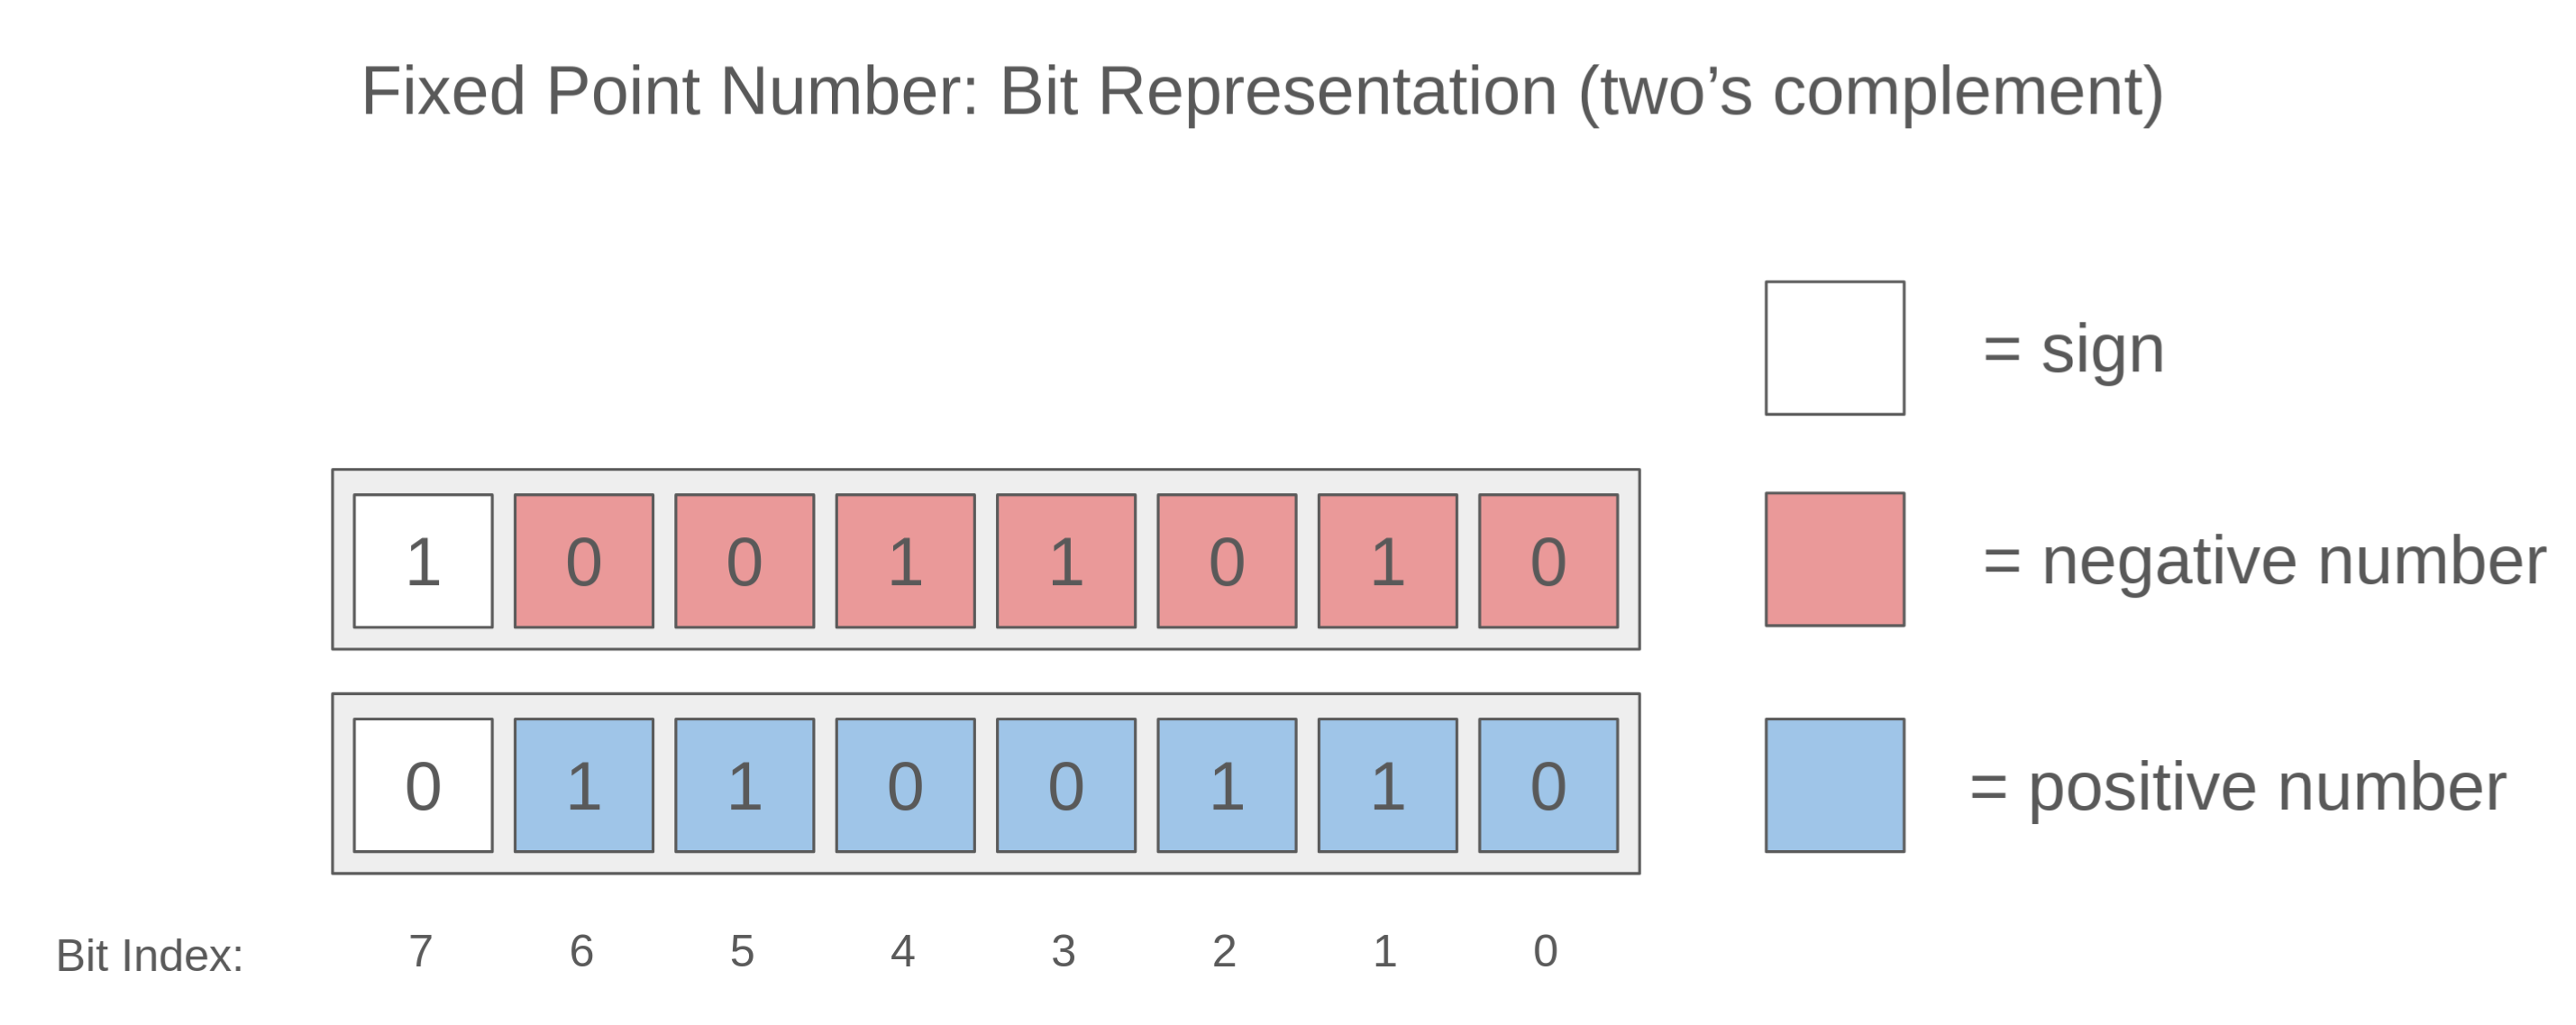
\includegraphics[width=0.5\linewidth]{Images/fixed_point_bit_representation.png}
    \caption{Fixed point representation of a number in binary. The figure shows one number and its complement, represented using the two's complement method.}
    \label{fig:fixed_point_representation}
\end{figure}

Fixed point numbers are represented by allocating a fixed amount of bits for the fractional part, and a fixed number of bits for the integer part. This is implicit and not visible in how a processor treats the numbers, which means that the processor can use the same hardware for operating on fixed point (fractional) numbers as regular integers, which is often speedier than performing operations on floating point numbers. It then becomes the programmers job to scale the number, often done by shifting the number to the left (which is equivalent to multiplying the number by $2^n$, $n$ being the amount of bits you are shifting the value.

Therefore, depending on the program, the numerical values for the bit representations in figure~\ref{fig:fixed_point_representation} could be 102 for the positive and -102 for the negative if we do not use a scaling factor, or if we decide that the three lower bits should be the fractional part of the number, to get our output number we must perform a right shift three places for the integer part of the number: 1100, which gives us the integer 12. The rightmost bits also have to be scaled by the same factor, i.e. $2^3$. To represent this as a decimal number requires us to divide by the scaling factor. 110 in binary is the same as 8 in integer representation. This gives us $6/8 = 0.75$, making the number represented 12.75.

Fixed point numbers can represent a smaller range of numbers with the same amount of bits as a floating point representation, and with lower precision. The flip side is that they are in general easier to perform computations on. 

\taffo therefore depends on users of the program to annotate a variable that is to be converted to a fixed point type with the range of values it can have, which is used to decide how many bits is required to represent the number accurately enough as a fixed point number. 

These two tools were selected as they were two of the few tools that had source code available on the internet without having to beg the authors in the paper for crumbs. 

There are other papers detailing different methods of approximate computing. Sadly, though they are described vividly in the papers, efforts to get a hold of these storied approximate computing tools proved fruitless. Though the tools described in the papers do not as far as I am concerned exist, the techniques exist, and can be applied manually.

\subsubsection{Approximate Computing through Loop Perforation}

Loop perforation, described in~\citet{li2018sculptor}, works by skipping iterations in loops that iteratively get closer to an accurate number. This would not necessarily work on just any loop, such as a loop reading in lines of data from a file, as this could cause data corruption.

\subsubsection{Approximate Computing through Memoization}

Memoization consists of mapping the inputs of expensive functions to their outputs, and avoiding to re-run the function for the same input, thereby saving energy. This is described more in depth in~\citep{mittal2016survey}.

\subsection{Fault Tolerance}

\subsubsection{Fault Tolerance Requirements}